\documentclass[journal]{IEEEtran}
\usepackage{amsmath,amsfonts}
\usepackage{algorithmic}
\usepackage{algorithm}
\usepackage{array}
\usepackage[caption=false,font=normalsize,labelfont=sf,textfont=sf]{subfig}
\usepackage{textcomp}
\usepackage{stfloats}
\usepackage{url}
\usepackage{verbatim}
\usepackage{graphicx}
\usepackage{cite}
\hyphenation{op-tical net-works semi-conduc-tor IEEE-Xplore}
% updated with editorial comments 8/9/2021

\begin{document}
\title{Title}
\author{Wenjin Xu, Chenguang Yang~\IEEEmembership{Fellow,~IEEE,}
    \thanks{This paper was produced by the IEEE Publication Technology Group. They are in Piscataway, NJ.}
    \thanks{Manuscript received April 19, 2021; revised August 16, 2021.}}

% The paper headers
\markboth{Journal of \LaTeX\ Class Files,~Vol.~14, No.~8, August~2021}%
{Shell \MakeLowercase{\textit{et al.}}: A Sample Article Using IEEEtran.cls for IEEE Journals}

% \IEEEpubid{0000--0000/00\$00.00~\copyright~2021 IEEE}
% Remember, if you use this you must call \IEEEpubidadjcol in the second
% column for its text to clear the IEEEpubid mark.

\maketitle
\begin{abstract}
In our daily life, human can accomplish complex tasks with great ease by inspiring and generalizing a set of fundamental skills from the past. Notably, it would be outstanding for the robotic control systems to benefit from such brilliant learning capability. In the last decades, many researchers have paid their massive efforts to investigate the robotic motor control learning problems to provide reasonable decision-making and advanced control methods, such as sliding mode control, adaptive NN control and robust control, etc. In general, it is well known that the robot dynamic is hard to be modeled appropriately with the increasing complexity of manipulator's structure. Due to the excellent approximation capability of NN and fuzzy system, they have been extensively utilized for adaptive control systems to estimate the unknown dynamic of robot at any specific accuracy. Particularly, a notable method which incorporates the fuzzy logic to adaptive NN control has been widely adopted to address the problems of lacking automatic learning capabilities in fuzzy system. By considering the uniform boundedness and state constraints, He~\textit{et al.} proposed an adaptive fuzzy neural network (FNN) control to address the interaction problem of robot. In, a developed FNN control structure is employed to approximate the uncertain dynamic model of a dual-arm robot. Despite much progress achieved in model approximation, several other methodologies have been proposed to ensure the control performance, such as input saturation which can tackle the control problem related to input constraint, finite-time
convergence control.
\end{abstract}

\begin{IEEEkeywords}
    robotic
\end{IEEEkeywords}

\section{Introduction}
\IEEEPARstart{D}{uring} the past few years, increasing robotic manipulator techniques have been employed into industrial applications and our daily life. One of the most difficult problems in robotic research is how to achieve the human-like working manner in its workspace, such as distinctive capability of skills learning and friendly desirable interaction control. Such abilities are of great importance to enable robots to respond more intelligently and be able to fulfil more complex, dexterous and versatile tasks in various fields such as industrial applications and service areas. 

Nevertheless, a key problem in the aforementioned control schemes which is tough to address is that the neural nodes for NN or the logic rules for fuzzy system are specified beforehand in terms of the expert experiences. Once the desired motion trajectory or working environment is changed, the original controller, unsurprisingly, may result in poor control tracking performance even irreversible consequence. In such case, the FNN controller, which is lack of generation ability from neural biological attribute point of view, needs to be redesigned to deal with the new tasks. Recently, a novel framework named broad learning system, which is developed from random vector functional-link neural networks (RVFLNN), has been proposed and extensively utilized for pattern recognition and classification. By taking the advantages of RVFLNN, BLS can offer acceptable generalization and efficient expansion performance through increasing the neural nodes dynamically. Herein, this inspires us to bring a forward solution which incorporates BLS to improve the generalizing ability of FNN.

As mentioned above, it is innate for humans to adjust the impedance and force of their arms skillfully while interacting with the unknown environments. From a biological point of view, humans can adapt their endpoint impedance of limbs through the central nervous system to achieve compliant interaction. Therefore, it would be crucial and significant to control robot in such way for a variety of social applications such as health care, assembly line and human-robot collaboration. In the literature, significant progress has been made to tackle such related issues. Generally, it is of great importance to establish a desired impedance model for impedance control parameters of which are difficult to choose from in practical. One of the most important parts of impedance control is to determine the desired impedance parameters. Nevertheless, most existing impedance control methods used fixed and manual designed impedance model. In order to improve the performance of compliant interaction under unknown environment, optimization of the impedance model should be taken into consideration. In, a desirable force regulation and tracking performance have been achieved by means of linear quadratic regulator (LQR), which is operated by considering a minimal cost function, to optimize the impedance parameters under a vital precondition of completely known environment dynamics. However, such algorithms seem too conservative to achieve a desired robot-environment interaction since they lack the ability of incorporating the unstructured and dynamic environments. Progress has been made in addressing such problems, and various optimal control schemes in the case of unknown environment have been proposed in literature. It proposed a force sensorless admittance control for robots to tackle with the unknown robot-environment interaction.

The main contributions of this article are listed as follows. \cite{Ju2012}.

1) We propose a learning method based on DMP and FGMM which can not only learn the trajectory from multiple demonstrations but also learn the deviation among them.

2) We present a new LfD method which can demonstrate by a single static image, each sample point on the image is encoded by a prior trajectory and FGMM. The skills are then learnt through the proposed methods.

3) We give a method for generating a priori trajectories of Chinese characters and design a robot learning framework for learning to write. Experiments were carried out on the LASA dataset and Chinese character images to verify the effectiveness of the method.

\begin{figure*}[!t]
    \centering
    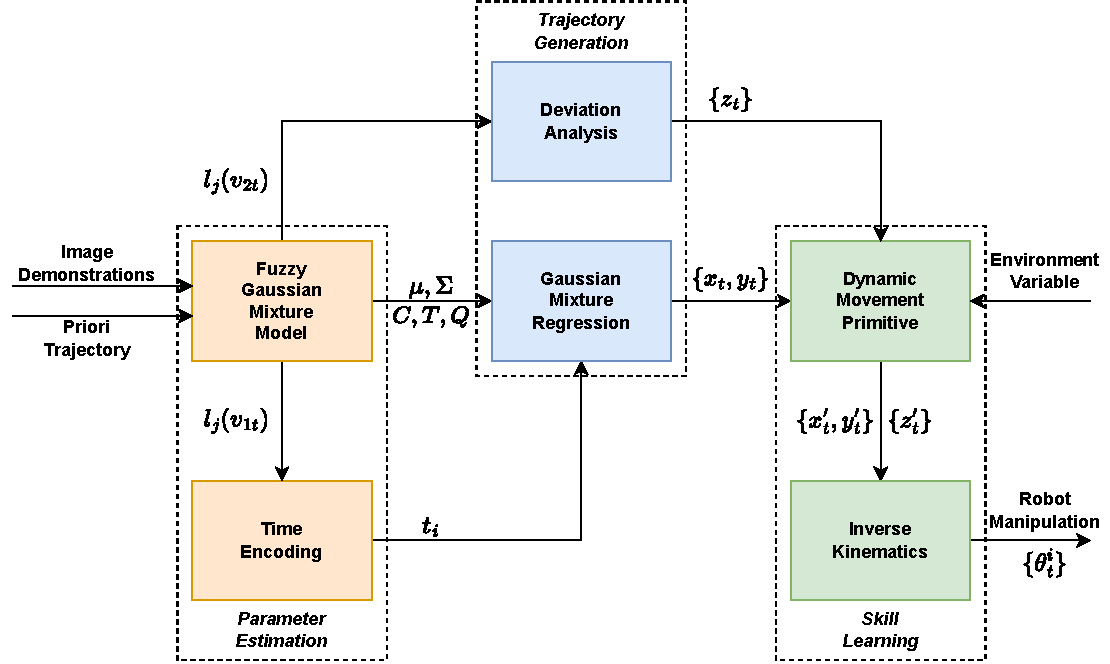
\includegraphics[width=6in]{./fig/fig1.pdf}
    \caption{Block diagram of the proposed system.}
    \label{fig1}
\end{figure*}

\section{Methodology}
\subsection{System Description}
The block diagram presented in Fig. \ref{fig1} illustrates the framework of the imitation learning system for robotic handwriting tasks. The system can learn skills from static images and prior trajectories, particularly focusing on the deviation information within them, and ultimately achieving skill generalization in various environments. The entire system encompasses three aspects:

1)~Image Demonstration: The demonstration part transfers the writing skill to the robot through the character image written by a human. The proposed system enables robot learning parameters of FGMM from a static image. On the other hand, the priori information of time is attained by the priori trajectories, which explicitly show the implicit time information in the image.

2)~Skill Learning: With the parameters estimated in the previous part, we can encode the writing skill through GMR. The normal GMR method can generate the trajectory very well. However, the effect of learning the deviation among samples in the image is not that good. Therefore, we proposed a novel approach called deviation analysis to enhance the deviation learning ability of GMR. 

3)~Motion Generalization: It is common to adjust the generalization effect of writing skills in different situations, like changing the size of the written font to adapt the various types of papers in the real world. DMP is used to make the skill have great generalization performance. DMP can encode not only the trajectory but also the end-effector orientation.

\subsection{Fuzzy Gaussian Mixture Model}
Gaussian Mixture Models have been widely applied in various fitting scenarios. However, due to the linearity of the axes in GMM, more components are required to fit nonlinear data. Paper \cite{Ju2012} introduce a modified GMM called Fuzzy Gaussian Mixture Model (FGMM). It combines the conventional GMM with Active curve axis Gaussian mixture models (AcaG)\cite{Zhang2005} and introduces a dissimilarity function to accelerate convergence. Fig. \ref{fig2} represents the data transformation process of FGMM.
\begin{figure}[!t]
    \centering
    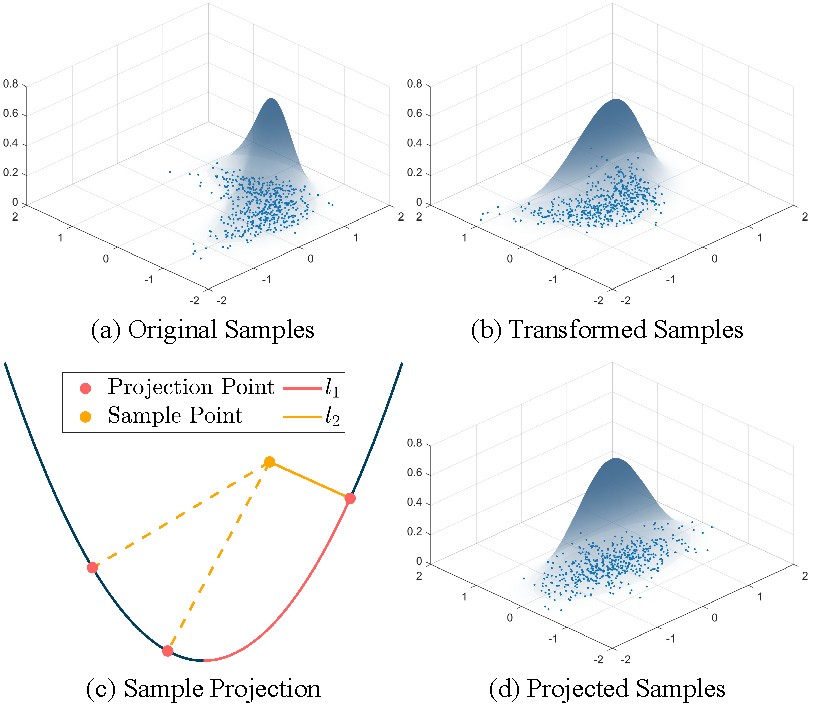
\includegraphics[width=3in]{./fig/fig2.pdf}
    \caption{The data transformation process of FGMM.}
    \label{fig2}
\end{figure}

$X=\{x_1,\hdots,x_N\}$ is a $d$-dimensional observed dataset with $N$ vectors. Normally, we assumed that the distribution of $X$ is based on the mixture Gaussian distribution, which the following equation can represent:
\begin{equation}
    p(x_n|\mu,\Sigma)=\sum\limits^K_{i=1}\alpha_i p_i(x_n|\mu_i,\Sigma_i)
\end{equation}  
where $x_n$ is a $d$-dimensional vector and $\alpha_i$, $\mu_i$, $\Sigma_i$ mean the $i^{th}$ Gaussian component's weight, mean and variance respectively. $K$ is a pre-set parameter representing the number of Gaussian components. However, the data with nonlinear characteristics do not fit this assumption well, like the data presented in Fig.\ref{fig2}a. AcaGMM introduces non-linear factors to the conventional GMM. In the following part, we introduce the definition and parameter estimation process of AcaGMM.

First, the k-means algorithm divides the dataset into $K$ classes. For each class of data, we transfer them to a new coordinate through PCA (Principal Component Analysis) :
\begin{equation}
    Y_i=Q_i \times (X_i-T_i)
\end{equation}
where $Q_i$ and $T_i$ denote the rotation matrix and translation vectors. $X_i$ is data which belongs to the $i^{th}$ components. The transformed data $Y_i$ presented in Fig.\ref{fig2}b have zero mean, and their principal axis aligns with the transformed x-axis. Noticed that we assume all data are two-dimensional in this paper. The LSFM (least-squares fitting method) is used to fit the data using a parabolic curve, which is defined as:
\begin{equation}
    y=cx^2+b
\end{equation}
where $c$ denotes the curvature of data and $b$ is the bias. Assuming all data satisfies the parabolic equation, the linear function can be written as:
\begin{equation}
    \left[
        \begin{array}{c}
            (y_1)^2\\
            (y_2)^2\\
            \vdots\\
            (y_n)^2\\
        \end{array}
    \right]=
    \left[
        \begin{array}{cc}
            (x_1)^2 & 1 \\
            (x_2)^2 & 1 \\
            \vdots & \vdots \\
            (x_n)^2 & 1 \\
        \end{array}
    \right]
    \left[
        \begin{array}{c}
            c\\
            b\\
        \end{array}
    \right]
\end{equation}
where the equation can be written as $Y=XC_i$. The least-squares solution is $C_i=(X^{\mathrm{T}}X)^{\dagger}X^{\mathrm{T}}Y$, where $\dagger$ means Moore–Penrose pseudoinverse. For components with small values of $c$, they can be degenerated into a conventional GMM:
\begin{equation}
    y=\left\{
    \begin{aligned}
        &b&(|c|<\epsilon)\\
        &cx^2+b&(|c|>\epsilon)\\
    \end{aligned}
    \right.
\end{equation}
where $\epsilon$ is a small positive number. If $|c|$ is smaller than $\epsilon$, the principal axis can be approximated as a straight line, and the component can be seen as a conventional GMM component.  Otherwise, if  $|c|$  is bigger than $\epsilon$, the component can be considered as an AcaGMM component.

AcaGMM uses the projection point on the parabolic curve to replace the sample point for calculating the posterior probability. First, the distance between a sample point $\{x_{1t},x_{2t}\}$ and its projection point $\{z_{1},z_{2}\}$ satisfies:
\begin{equation}
    \begin{aligned}
    d^2&=(z_{1}-x_{1n})^2+(z_{2}-x_{2n})^2 \\
    z_2&=cz_1^2+b
    \end{aligned}
\end{equation}

The Lagrange method is used to find the closest projection point:
\begin{equation}
    2c^2z_1^3+(2bc-2cx_{2n}+1)z_1-x_{1n}=0
\end{equation}
the cubic function may have multiple solutions, which means a sample may have multiple projection points with the shortest distance. Then we calculate the arc length of the $j^{th}$ projection points $\{z_{1j},z_{2j}\}$:
\begin{equation}
    l_{1j}=\int_{(0,b)}^{(z_{1j},z_{2j})}\sqrt{(dz_{1j})^2+(dz_{2j})^2}
\end{equation}
eliminate $z_{2j}$, we have:
\begin{equation}
    l_{1j}=\frac{1}{2}z_{1j}\sqrt{4c^2z_{1j}^2+1}+\frac{1}{4|c|}ln(2|c|z_{1j}+\sqrt{4c^2z_{1j}^2+1})
\end{equation}
and the distance between $x_t$ and $z_j$ is:
\begin{equation}
    l_{2j}=\sqrt{(x_{1t}-z_{1j})^2+(x_{2t}-z_{2j})^2}
\end{equation}
where fig \ref{fig2}c illustrates the geometric meaning of $l_{1j}$ and $l_{2j}$.

Then we can calculate the probability of the sample $x_t$ via the sum of its projection points $z_j$:
\begin{equation}
    p_i(x_n|\theta_i)=\sum\limits^{J_t}_{j=1}\frac{exp(-l_{1j}^2/2\Sigma_1-l_{2j}^2/2\Sigma_2)}{2\pi\sqrt{|\Sigma_1\Sigma_2|}}
\end{equation} 
where the parameter $\theta_i=(\mu_i,\Sigma_i,C_i,Q_i,T_i)$, and $J_t$ means the number of projection points of the sample $x_n$.  

The EM algorithm is proposed for parameter estimation in AcaGMM. Due to the change in the probability density function, the parameter estimation method of AcaGMM differs from the conventional GMM. The procedure of the new EM algorithm is:

1) E-step: For each component, calculate the "expected" components of all samples:
\begin{equation}
    w_{in}=\frac{\alpha_ip_i(x_n|\theta_i)}{\sum^k_{s=1}\alpha_sp_s(x_n|\theta_s)}
\label{eq1}
\end{equation}
where $w_{in}$ denotes $x_n$ posterior probability for the $i^{th}$ components.

2) M-step: For each component, calculate the maximum likelihood of the given sample. The weight of each component is then estimated from:
\begin{equation}
    \alpha_i=\frac{1}{N}\sum\limits^N_{n=1}w_{in}
\end{equation}

Then parameters $C_i,T_i,Q_i$ can be estimated from:
\begin{equation}
    (C^{new}_i,T^{new}_i,Q^{new}_i)=LSFM(PCA(X_i))
\end{equation}
where $X_i$ denotes samples belonging to the $i_{th}$ components, which can be classified by Eq. \ref{eq1}. $\mu_i$ can be estimated by the following method:
\begin{equation}
    \mu_i^{new}=\frac{\sum^N_{n=1}w_{in}x_n}{\sum^N_{n=1}w_{in}}+(Q_i^{new})^{\bf{T}}[0,b]^{\bf{T}}+T_i^{new}
\end{equation}
and $\Sigma_i$ can be estimated from:
\begin{equation}
    L_{sn}=\frac{\sum^{J_{in}}_{j=1}p(l^i_{sj}|0,\Sigma^{old}_{si})l^i_{sj}}{\sum^{J_{in}}_{j=1}p(l^i_{sj}|0,\Sigma^{old}_{si})}~(s=1,2)
\end{equation} 
\begin{equation}
\Sigma_{si}=\frac{\sum_{n=1}^Nw_{in}L_{sn}}{\sum_{n=1}^Nw_{in}}~(s=1,2)
\end{equation}
where $L_{1n}$ denotes the mean arc length of $x_n$'s projection points, and $L_{2n}$ means the average distance between $x_n$ and its projection points. It can be considered that samples $X_n$ undergoes a non-linear transformation to obtain $L_n=\{L_{1n},L_{2n}\}$, presented in Fig.\ref{fig2}d. $L_n$ satisfied the distribution of the conventional zero-mean Gaussian.

The above step represents a single iteration of the EM algorithm. Repeat the iteration and update the parameters until the relative difference of log-likelihood between two iterations is less than a preset threshold. FGMM introduces an FCMs (Fuzzy C-means) mechanism to accelerate the convergence speed of the EM algorithm. 

\subsection{Time Encoding}
Traditional vision-based demonstrations are mostly obtained by recording motion sequences to acquire demonstration trajectories. Data usually contains time sequences, and time-driven methods like GMR and DMP are used for motion encoding and skill learning. However, in some scenarios, the time sequence of demonstration trajectories is missing, like demonstrating writing skills through an image. A new method based on FGMM is proposed for encoding the time series of demonstration trajectories.
\begin{figure}[!t]
    \centering
    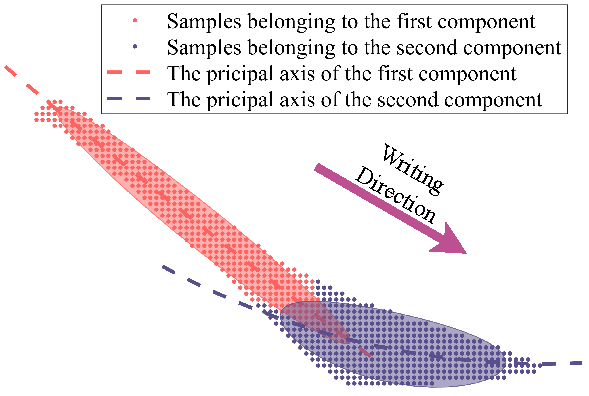
\includegraphics[width=3in]{./fig/fig3.pdf}
    \caption{Fitting Chinese stroke using FGMM.}
    \label{fig3}
\end{figure}

First, estimate the parameter of FGMM using the EM algorithm proposed before. Here we use a Chinese character stroke image as an example, presented in Fig.\ref{fig3}. The direction is needed to determine a general direction of movement. The direction does not need to be very precise. Most Chinese character strokes follow a sequence from left to right and from top to bottom, so the order of FGMM components can be determined. Each sample has a transformed point $L_n$ after a non-linear transformation during the parameter estimation. For most writing tasks involving movement along the principal axis, time information can be obtained through $L_{1n}$, which denotes the relative position of the sample on the principal axis. First we transfer the transformed sample from the first component $L_{1}^{(1)}=\{L_{11}^{(1)}, \hdots, L_{1n}^{(1)}\}$ to a zero starting point:
\begin{equation}
    t^{(1)}=\{L_{11}^{(1)}, \hdots, L_{1n}^{(1)}\}-min(L_{1}^{(1)})
\end{equation}

For the second component of transformed sample $L_{1}^{(2)}$, transfer them to the end of the first sequence:
\begin{equation}
    t^{(2)}=\{L_{11}^{(2)}, \hdots, L_{1n}^{(2)}\}-min(L_{1}^{(2)})+max(L_{1}^{(1)})
\end{equation}
if there are multiple components, repeat this process until the end. The time sequence is denoted as $\{t^{(1)},t^{(2)},\hdots,t^{(i)}\}$. Fig.\ref{fig4} presents the result of time encoding. The arrow on the sample point indicates the direction of time flow.
\begin{figure}[!t]
    \centering
    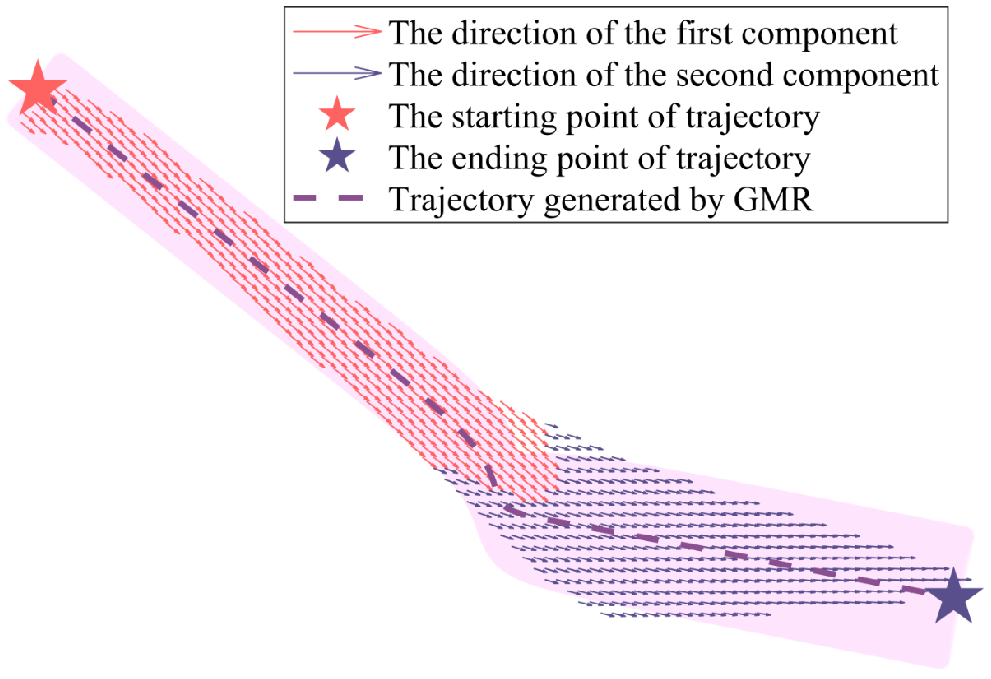
\includegraphics[width=3in]{./fig/fig4.pdf}
    \caption{The result of time encoding and GMR.}
    \label{fig4}
\end{figure}

\subsection{Gaussian Mixture Regression}
After time encoding, the time-driven method can be used for motion planning in writing tasks. Gaussian Mixture Regression (GMR) is a statistical learning technique that combines the GMM with linear regression. GMR is used to address nonlinear regression problems by capturing the intrinsic structure of the data through a Gaussian mixture model, which is then used to perform regression analysis. GMR allows us to specify one dimension of the GMM as input, with the remaining dimensions as output. Here, the time sequence $t$ obtained before is used as the input, and the position $X=\{x_1,\hdots,x_n\}$ as the output to plan the writing trajectory. The regression function can be considered as obtaining the expectation of an event for the output $X$ conditional on the input $t$:
\begin{equation}
    \mathcal{F} _{gmr}(t)=E(X|t)
\end{equation}

Assume that $X$ and $t$ follow the Gaussian distribution, the event satisfies:
\begin{equation}
    X|t \sim G(\mu_X+\frac{\sigma_{21}}{\sigma_{1}}(t-\mu_t),\sigma_{2}-\frac{\sigma_{12}\sigma_{21}}{\sigma_{1}})
\end{equation}
where $\sigma_{1}$ and $\sigma_{2}$ denote the variance of $t$ and $X$, $\sigma_{12}$ and $\sigma_{21}$ denote the covariance between $t$ and $X$. Consider that the Gaussian mixture model can be seen as a linear combination of Gaussian distributions, the expectation can be written as:
\begin{equation}
    \mathcal{F} _{gmr}(t)=\sum\limits_{i=1}^{K}w_i(t)\eta_i(t)
\end{equation}
where
\begin{equation}
    w_i(t)=\frac{\alpha_{i}G(t|\mu_{i}(t),\sigma_{it})}{\sum_{i=1}^{K}\alpha_{i}G(t|\mu_{i}(t),\sigma_{it})}
\end{equation}
\begin{equation}
    \eta_i(t)=\mu_{iX}+\frac{\sigma_{21i}}{\sigma_{1i}}(t-\mu_{it})
    \label{eq2}
\end{equation}

In the previous part, the GMM is replaced with FGMM, which has better non-linear fitting capability. The regression function should be redesigned. Paper\cite{Yang2019c} proposes a new regression algorithm for FGMM. Notice that Eq.\ref{eq2} is a linear function, it defines the location of GMM's principal axis. For the FGMM, the corresponding axis can be obtained from the PCA inverse transformation:
\begin{equation}
    A_i'=Q_i^{\bf{T}}A_i+T_i
\end{equation}
where $A_i$ and $A_i'$ denote the original axis and transformed axis. The regression for FGMM can be denoted as:
\begin{equation}
    \mathcal{F}' _{gmr}(t)=\sum\limits_{i=1}^{K}w_i'(t)A_i'
\end{equation}
where the FGMM component should replace each Gaussian component in $w_i'$, the movement trajectory planning by GMR is presented in Fig.\ref{fig4}. Compared with Fig.\ref{fig3}, it can be seen that the trajectory highly overlaps with the principal axis.

\subsection{Deviation Analysis}
In some scenarios, such as transferring writing skills to robots, they need to learn not only the trajectory information of sample points but also the deviation among them. The pink area shown in Fig.\ref{fig4} denotes the covariance of trajectory generated by GMR. The fitting effect is not ideal. A new method based on FGMM is proposed. Analyse the deviation of samples to generate a variance sequence for a better fitting effect.

In addition to generating a trajectory from time input, GMR can also generate a corresponding covariance sequence $\{\Sigma_1,\hdots,\Sigma_t\}$. It denotes the covariance among samples in time $t$. The covariance matrix implicitly contains the posture and deviation of the trajectory. They can be obtained by eigenvalue decomposition:
\begin{equation}
    \Sigma_t=R_tD_tR_t^{-1}
\end{equation}
where $D_t$ and $R_t$ represent the eigenvalues and eigenvectors of the covariance matrix, respectively. According to the geometric meaning of eigenvalue decomposition, they also represent the scaling effect and rotation effect of the covariance matrix, respectively, which represent the deviation and posture information of the trajectory. $L_{2n}$ defines the distance between the transformed sample and the principal axis. It can be used to define a new scaling matrix. According to the $3\sigma$ rule, the new scaling matrix is defined as:
\begin{equation}
    D_t^{new}=\left[
        \begin{array}{cc}
            (\frac{1}{3}L_{2t})^2&0\\
            0&D_{22t}
        \end{array}
    \right]
\end{equation}
the new covariance sequence is:
\begin{equation}
    \Sigma^{new}_t=R_tD^{new}_tR_t^{-1}
\end{equation}

\subsection{Dynamic Movement Primitive}
The DMP is a LfD model based on dynamic systems\cite{Ijspeert2013}. It consists of a second-order dynamic system and a non-linear function, allowing it to encode motion trajectories with fewer parameters while maintaining stability. For the encoded trajectory, modifying the positions of the starting and ending points can also retain the original motion characteristics:
\begin{equation}
    \ddot y = \alpha(\beta(g-y)-\dot y) + f
    \label{eq4}
\end{equation}

To change the trajectory speed, a scaling term $\tau$ is added in front of the velocity variable $\dot y$:
\begin{equation}
    \tau^2 \ddot y = \alpha(\beta(g-y)-\tau \dot y) + f
\end{equation}

To decouple the non-linear equation from time, a canonical system $x(t)$ is used to drive the dynamic system:
\begin{equation}
    \tau \dot x = - \kappa x
\end{equation}

The first term in Eq.\ref{eq4} is a PD (Proportional-Derivative) system. To avoid overshooting and ensure stable convergence to the attractor, let the parameter $\beta = \alpha / 4$, rewriting the second-order dynamic system as a critically stable spring-damping system. The system ultimately converges stably to the position $g$. The second term $f$ in Eq.\ref{eq4} is a non-linear function that controls the intermediate process of convergence. The non-linear function $f$ can be expressed as:
\begin{equation}
    f(x)=\frac{\sum\limits_{i=1}^{N} \Psi_{i}(x) w_{i}}{\sum\limits_{i=1}^{N} \Psi_{i}(x)}x(t)(g-y)
    \label{eq5}
\end{equation}
where, $\Psi(t)$ is a Radial Basis Function (RBF), expressed as:
\begin{equation}
    \Psi_i(x)= \exp \left(-\frac{\left(x-\mu_i \right)^{2}}{2 \sigma_i^{2}}\right)
\end{equation}
where $N$ represents the number of RBF, $\mu_i$ represents the position of the $i^{th}$ basis function, and $\sigma_i$ represents the width of the $i^{th}$ basis function. $\omega_i$ represents the weight of the $i^{th}$ radial basis function, which needs to be obtained by learning from the demonstration trajectory. Given a demonstration trajectory $y_{dms}$, the expression for $f_{dms}$ can be derived from Eq.\ref{eq4}:
\begin{equation}
    f_{dms} = \tau^2 \ddot y_{dms} - \alpha(\beta (g-y_{dms})-\tau \dot y_{dms})
    \label{eq6}
\end{equation}
where Locally Weighted Regression (LWR) is used to determining the weight parameter $w_{i}$, which can control the $f(x)$ to fit $f_{dms}$.

\section{Experiments}
\subsection{Simulation}
In this part, The proposed method is verified through simulation. A Chinese calligraphy image is used as the demonstration image, denoted in Fig.\ref{fig1}. Paper \cite{Li2022} propose an observation based method which can extract strokes from the Chinese character image. The result is represented in Fig.\ref{fig1}. It divides Chinese characters into several strokes and indicates their writing direction. Then 


\section{Conclusion}
\bibliographystyle{IEEEtran}
\bibliography{IEEEabrv,reference.bib}
\end{document}


